\documentclass[times, utf8, zavrsni, numeric]{fer}
\usepackage{booktabs}
\usepackage{caption}
\usepackage{hyperref}
\usepackage{rotating}
\usepackage{microtype}
\usepackage{afterpage}

\begin{document}

\thesisnumber{6848}

\title{Podržana evolucija agenta za igru Dota 2}

\author{Jakov Ivković}

\maketitle

% Ispis stranice s napomenom o umetanju izvornika rada. Uklonite naredbu
% \izvornik ako želite izbaciti tu stranicu.
\izvornik{}

% Dodavanje zahvale ili prazne stranice. Ako ne želite dodati zahvalu, naredbu
% ostavite radi prazne stranice.
\zahvala{Zahvaljujem se mentoru prof.~dr.~sc.~Domagoju~Jakoboviću na vrlo
zanimljivoj temi te podršci tijekom izrade rada.

Zahvaljujem se kolegici Lauri Torić na dragocjenim savjetima te na međusobnoj
razmjeni ideja.} 

\tableofcontents

\chapter{Uvod}

Rad se bavi problemom s GECCO 2020\footnote{The Genetic and Evolutionary
Computation Conference} natjecanja naziva \emph{Dota 2 1-on-1 Shadow Fiend
Laning Competition}.  Cilj natjecanja je izraditi što boljeg agenta za
računalnu MOBA\footnote{Multiplayer Online Battle Arena} igru Dota 2 u 1v1
formatu.

Problemu će se pristupiti koristeći evolucijske algoritme; evolucijska
strategija i genetski algoritam te dva različita modela jedinke; neuronska
mreža i CGP\footnote{Kartezijsko genetsko programiranje \engl{Cartessian
Genetic Programming}}.  Jedinke ćemo evaluirati s obzirom na odluke koje donose
tijekom igre.

U poglavlju~\ref{chapter:opis-problema} nalazi se kratki pregled pravila igre te
opis problema. Nakon toga, u poglavlju~\ref{chapter:implementacija} nalazi se
opis svih komponenti programskog rješenja te osvrt na njihovu implementaciju. Na
kraju, u poglavlju~\ref{chapter:rezultati} je opis postignutih rezultata te,
nakon toga, u poglavlju~\ref{chapter:zakljucak} zaključak temeljen na tim
rezultatima.

\chapter{Opis problema}\label{chapter:opis-problema}

\section{DotA}

DotA\footnote{Defense of the Ancients} je MOBA igra koja je nastala 2003.\
godine kao mod za stratešku igru Warcraft III.\@ 10 godina kasnije, 2013.\
godine izlazi Dota 2. Zapravo potpuno ista igra, samo u standalone verziji s
boljom grafikom i kontrolama.

Izlaskom Dote 2 popularnost igre raste te do danas Dota ostaje jedna od
najpopularnijih\footnote{Preko 8 milijuna MAU \engl{Monthly Active Users}} igri
u MOBA žanru.  Također, zbog svoje kompleksnosti Dota ubrzo postaje
najkompetitivnija igra u esports svijetu s dotad neviđenim nagradnim fondovima
na turnirima. Samo prošlo svjetsko prvenstvo (pod imenom \emph{The International
9}) imalo je ukupan nagradni fond od nešto više od 34 milijuna američkih
dolara.\citep{liquipedia-ti9}

Izrazita kompleksnost igre zainteresirala je i računalne znanstvenike te su,
2017.\ godine, znanstvenici iz neprofitne organizacije OpenAI izradili agenta za
1v1 inačicu Dote sa \emph{Shadow Fiend} herojem\footnote{Heroji --- Likovi koje
igrači kontroliraju \engl{Hero}.}, što je upravo problem kojim se bavi i ovaj
rad. Agent je vrlo brzo savladao najbolje svjetske
igrače\citep{openai-1v1}, međutim, 1v1 je
egzibicijski mod i kompleksnošću nije ni blizu standardnom 5v5 Dota formatu.
Stoga, već godinu dana kasnije, 2018.\ godine OpenAI je izradio \emph{OpenAI
Five} --- 5 nezavisnih agenata koji zajedno igraju u standardnom\footnote{uz
određena ograničenja} 5v5 formatu.  Ubrzo je OpenAI Five počeo pobjeđivati
naprednije igrače i amaterske timove, a već godinu dana kasnije pobijedio je i
svjetske prvake.\citep{openai-five}

\subsection{Pravila}

Dota se sastoji od mnogo mehanika koje ju čine kompleksnom. U ovom poglavlju
ćemo se dotaknuti samo najbitnijih mehanika za ovaj rad.

Dota se igra s 10 igrača koji su suprotstavljeni u dva tima po 5 igrača.  Svaki
igrač kontrolira svog heroja.  Ukupan broj heroja je 119 te svaki igrač, na
početku meča, bira kojeg će igrati.  Heroji se međusobno razlikuju po moćima
koje posjeduju te zbog toga zahtijevaju različite taktike kod igranja.  Svaki
tim pokušava nadvladati protivnički tim kako bi mu uništio bazu čime meč
završava.  Trajanje jednog Dota meča je uglavnom između 20 minuta i sat vremena
s prosječnim trajanjem od pola sata.

Baze dvaju timova povezane su preko 3 \emph{lanea}\footnote{3 trake, puteljka
\engl{lane}}, kao što je to vidljivo na slici~\ref{fig:moba-map}. Na svakom
laneu postoje po 3 obrambena tornja (plavi i crveni kružići na slici) koje je
potrebno uništiti kako bi se došlo do protivničke baze. Svakih 30 sekundi se u
bazama stvaraju po 3 vala \emph{creepova}\footnote{Slabi, nekontrolabilni
likovi} koji putuju po laneovima prema protivničkoj bazi.

\begin{figure}[h] 
    \centering
    \includegraphics[width=7cm]{img/Map_of_MOBA}
    \caption{MOBA map\\ \textsl{\scriptsize
    \href{https://creativecommons.org/licenses/by-sa/3.0/deed.en}{CC BY-SA 3.0}
    --- Original by
    \href{https://commons.wikimedia.org/wiki/User:Raizin}{Raizin}, SVG rework by
    \href{https://commons.wikimedia.org/wiki/User:Sameboat}{Sameboat}}}\label{fig:moba-map}
\end{figure}

\begin{figure}[h] 
    \centering
    \includegraphics[width=8cm]{img/tower-creeps}
    \caption{Toranj i val creepova}\label{fig:tower-creeps}
\end{figure}

\begin{figure}[h] 
    \centering
    \includegraphics[width=7cm]{img/creeps-mid}
    \caption{Borba creepova}\label{fig:creep-fight}
\end{figure}

Dva vrlo bitna faktora na koja igrači moraju paziti, o kojima ovisi jačina
njihovih heroja, su zlato \engl{gold} i iskustvo \engl{experience}. Svi heroji
na početku meča prilično su slabi te, pošto nisu sposobni napasti protivničku
bazu, vrlo velik naglasak u meču je upravo u borbi za ta 2 resursa. U velikoj
većini mečeva onaj tim koji ima značajnije veći posjed zlata i iskustva na kraju
i pobjedi.


Iskustvo određuje herojev \emph{level}. Heroji počinju s levelom 1 te su sa
svakim levelom jači (maksimalni level je 30). Heroji zarađuju iskustvo kada u
njihovoj blizini\footnote{U točno određenom radiusu prikazanom zelenom kružnicom
na slici~\ref{fig:exp-range}} umre neprijateljski lik\footnote{Bilo
neprijateljski creep ili neprijateljski heroj}.


Drugi bitan resurs je zlato. Glavni izvor zlata je \emph{last hitanje} creepova.
Last hit\footnote{zadnji udarac \engl{last hit}} je zadavanje zadnjeg udarca
neprijateljskom creepu. Ako igrač uspije zadati zadnji udarac creepu, dobit će
određenu količinu zlata kao nagradu. Igrač zlato koristi kako bi kupovao
\emph{iteme}, predmete koji dodatno ojačavaju heroja.


Vrlo bitna mehanika u doti, kojom se pokušava usporiti napredovanje protivnika,
je \emph{denyjanje} \engl{deny}. Denyjanje je last hitanje vlastitih creepova.
Denyjanjem igrač ništa ne dobiva za sebe, međutim, time onemogućuje
neprijateljskom heroju da dobije last hit nad tim creepom. Također, ako je creep
denyjan, on neprijateljskim herojima daje upola manje iskustva.

\begin{figure}[h] 
    \centering
    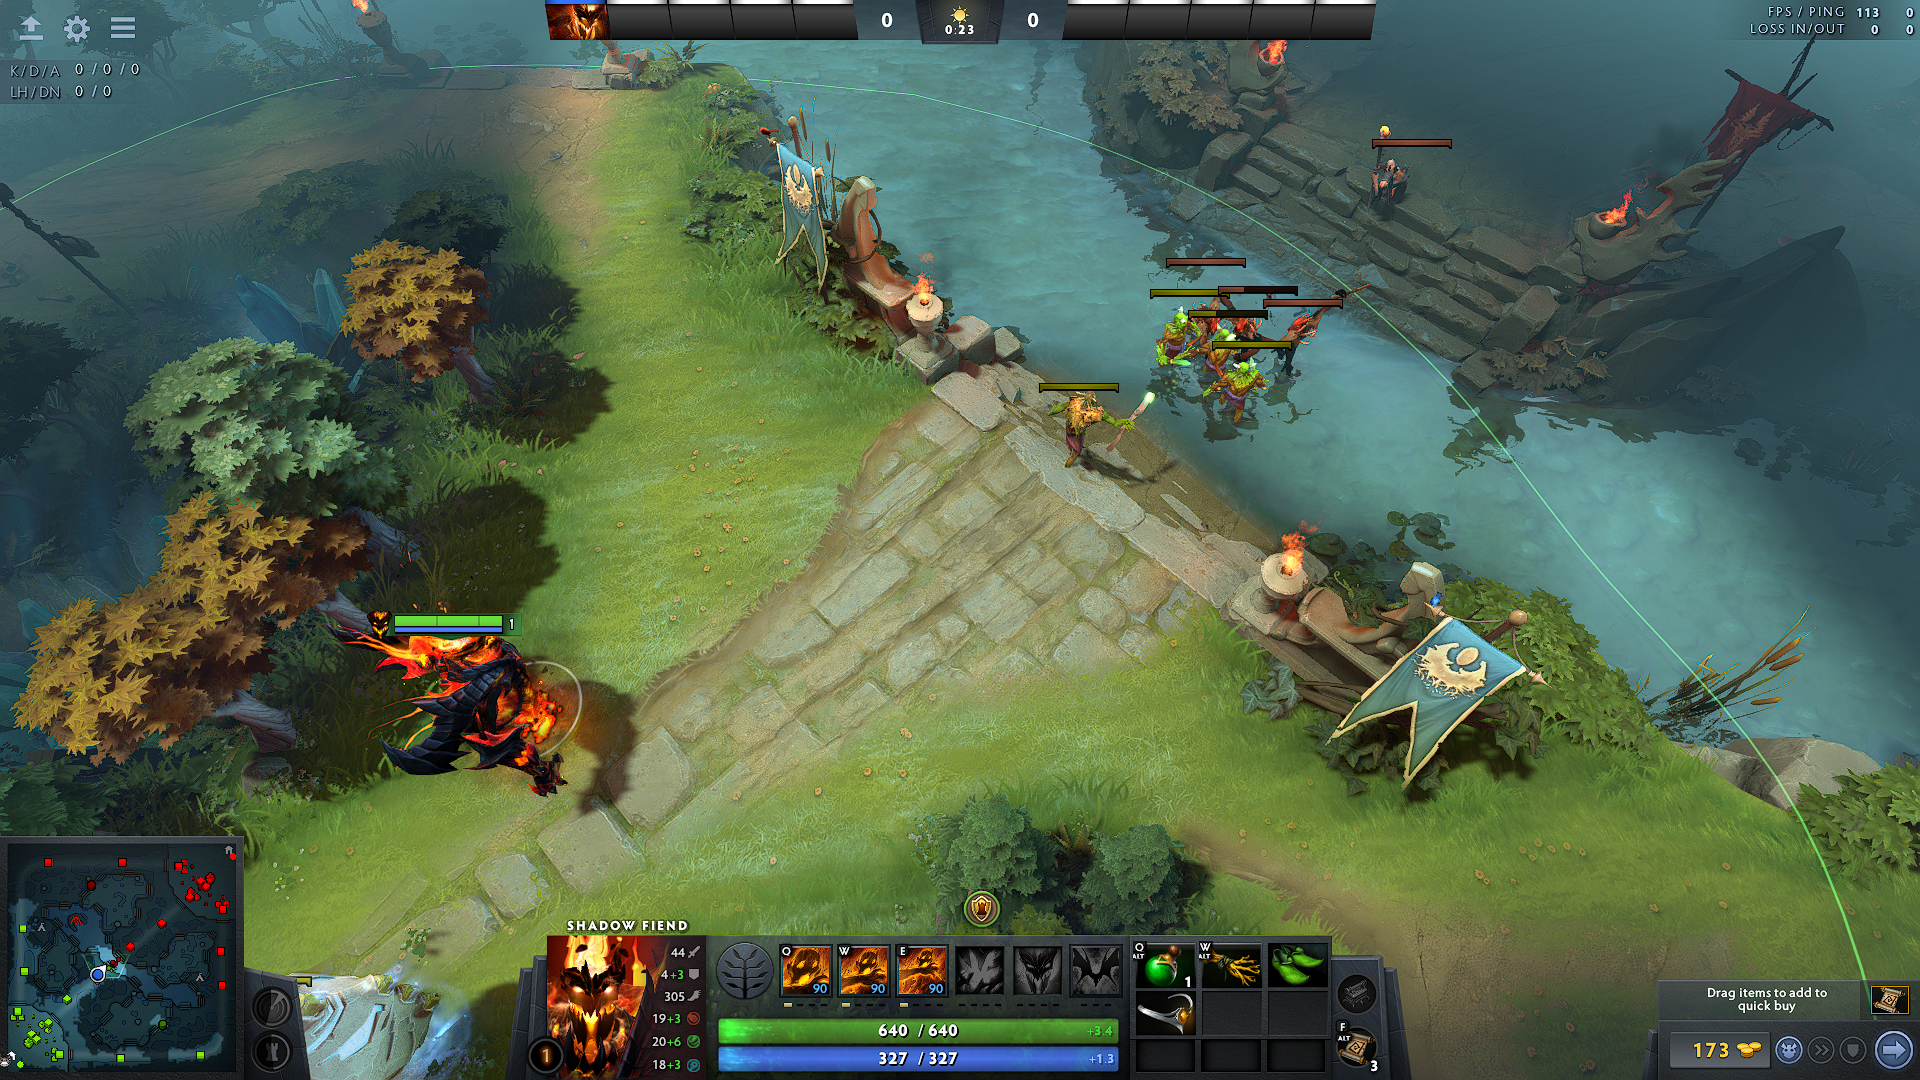
\includegraphics[width=13cm]{img/exp-range}
    \caption{Radius za iskustvo}\label{fig:exp-range}
\end{figure}

\begin{figure}[h] 
    \centering
    \includegraphics[width=7cm]{img/last-hit}
    \caption{Igrač (dolje desno) pokušava last hitati protivničkog creepa
    napadajući ga dok mu je \emph{health} nizak.}\label{fig:last-hit}
\end{figure}

\section{1v1 Shadow Fiend}

1v1 format mnogo je jednostavniji od standardnog 5v5 formata. Za razliku od
standardnog formata gdje se pobjeđuje uništavanjem protivničke baze, u 1v1
formatu pobjeđuje prvi igrač koji ubije protivničkog igrača dva puta ili prvi
koji uništi protivnički toranj na srednjem \engl{middle} laneu (pogledati
sliku~\ref{fig:moba-map}). Također, ostali laneovi su ``isključeni'' tako da se
na njima ne stvaraju creepovi te se tornjevi na njima ne mogu uništiti.
Dodatno, oba igrača igraju istog heroja, Shadow Fienda.

Shadow Fiend ima četiri različite moći od kojih ćemo proučiti dvije najvažnije
za ovaj format.

\subsection{Shadowraze}\label{shadowraze}

Shadowraze je moć koja se sastoji od tri \emph{podmoći} koje se mogu nezavisno
koristiti. Shadowraze čini veliku štetu neprijateljima u malom radiusu ispred
Shadow Fienda. Tri podmoći su identične s jedinom razlikom udaljenosti tog
radiusa od Shadow Fienda. Ova moć ima veliku korist kod uspješnog last hitanja
creepova te kod napadanja protivnika. Vrlo bitna stvar na koju igrač mora
paziti kod korištenja ove moći je orijentacija heroja. Nažalost, u Breezy
serveru je postojala greška zbog koje je agent dobivao pogrešne informacije o
svojoj orijentaciji te orijentaciji protivnika tako da agenti koji su trenirani
u sklopu rada nisu mogli uspješno naučiti koristiti, a ni izbjegavati
protivnički, Shadowraze.

\subsection{Necromastery}

Necromastery je pasivna moć koja povećava štetu udarca Shadow Fienda za svaki
last hit ili deny koji napravi. Ova moć, posebno u 1v1 formatu, stvara učinak
snježne grude \engl{snowball effect}.  Što heroj više last hita i denyja to će
stvarati veću štetu kod udaraca. Što heroj stvara veću štetu to mu je lakše
last hitati i denyjati. Zbog ove moći je izrazito veliki naglasak na što
efikasnijem last hitanju te denyjanju.  Onaj igrač koji bolje last hita i
denyja ima puno bolje izglede za pobijediti.

\begin{figure}[h] 
    \centering
    \includegraphics[width=15cm]{img/shadowraze}
    \caption{Sve tri Shadowraze podmoći\\ \textsl{\scriptsize
    \href{https://steamcommunity.com/sharedfiles/filedetails/?id=113306813}{Nubtrain
    --- Nevermore --- The Soultrain Stealer}}}\label{fig:Shadowraze}
\end{figure}

\section{Breezy}

Breezy je HTTP\footnote{Hyper Text Transfer Protocol} server i klijent koji
agentu služi kao sučelje prema igri. Upute za postavljanje servera mogu se naći
na stranici natjecanja.\citep{project-breezy}

Kako bi započeli igru, trebamo poslati POST zahtjev Breezy serveru na rutu
\textls{/run/}. U tijelu zahtjeva, u JSON\footnote{JavaScript Object Notation}
formatu, šaljemo broj mečeva koliko ih želimo pokrenuti. Nakon toga, Breezy
server pokreće igru te periodički šalje značajke igre agentu. Breezy server
šalje 310 značajki putem POST zahtjeva na predefiniranu rutu na agentu. Agent
zatim odgovara na te zahtjeve jednom od 30 dostupnih akcija.\footnote{Popis
značajki može se pogledati na
\href{https://app.swaggerhub.com/apis-docs/aianta/breezy-server/0.0.1\#/default/get\_features\_}{dokumentaciji
Breezy servera}, a dostupne akcije na
\href{https://web.cs.dal.ca/~dota2/?page\_id=353}{stranici natjecanja}.} Agent
igra protiv hardkodiranog \emph{bota} koji je dostupan u igri te koji je težine
\emph{hard}.\footnote{Botovi dostupni u igri imaju više dostupnih težina:
pasivan \engl{passive}, lagan \engl{easy}, srednje težak \engl{medium}, težak
\engl{hard} i nepošten \engl{unfair}} Kada dođe do kraja igre, Breezy server
šalje informacije o kraju igre putem POST zahtjeva na predefiniranu rutu na
agentu. Ako je ostalo još mečeva za odigrati\footnote{Ako smo kod prvotnog
zahtjeva prema Breezy serveru označili da želimo pokrenuti više od jednog meča},
u tijelu tog zahtjeva nalazit će se webhook ruta na Breezy serveru na koju treba
poslati GET zahtjev kako bi započeo novi meč.

\begin{figure}[h] 
    \centering
    \includegraphics[width=15cm]{img/breezy}
    \caption{Interakcija Breezy servera i agenta}\label{fig:breezy}
\end{figure}

Tri vrlo otežavajuća faktora agentima su nepoznavanje orijentacije svog ni
protivničkog heroja, nemogućnost denyjanja te veliki vremenski razmak između
dvije akcije.
\begin{itemize}
    \item Kao što je već spomenuto u poglavlju~\ref{shadowraze}, postojala je
        greška u Breezy serveru zbog koje značajke za orijentacije heroja nisu
        radile te, radi toga, agenti nisu mogli naučiti koristiti ni izbjegavati
        Shadowraze moć.\footnote{Značajke za orijentacije su ispravljene
        sljedećim git commitom:
        https://gitlab.com/LivinBreezy/project-breezy/-/commit/e86d0a8a3a892182817892867a525941a7bb47f4}
    \item Druga greška u Breezy serveru je nemogućnost denyjanja. Naime akcije
        za denyjanje creepova (njih 5), tijekom izrade rada, nisu
        radile.\footnote{Akcije su ispravljene sljedećim git commitom:
        https://gitlab.com/LivinBreezy/project-breezy/-/commit/078583ce5b19bc152995c1561eb173d4091fb560}
    \item Treći otežavajući faktor je brzina kojom Breezy server šalje značajke.
        Latencija od Breezy servera do igre je \textasciitilde110ms. Sama igra
        je ubrzana deset puta, odnosno jedna sekunda stvarnog vremena je 10
        sekundi u igri. Zbog velike latencije između Breezy servera i igre,
        Breezy server šalje, otprilike, 9 značajki po sekundi. S obzirom na to
        da je igra ubrzana deset puta, to znači da agent prima značajke i donosi
        akcije u razmacima od, otprilike, 0.1 sekunde stvarnog, odnosno 1
        sekunde vremena u igri.
\end{itemize}


Postoje dvije mehanike igre na koje agent ne mora paziti; ``levelanje'' moći te
kupovanje itema.\citep{project-breezy} Kod svakog novog levela kojeg heroj
dosegne, igrač mora odabrati moć heroja koju želi unaprijediti. Agent o tome ne
mora brinuti jer breezy server ima točno određeni redoslijed unaprjeđivanja moći
te automatski, kod svakog novog levela heroja, bira moć za unaprjeđivanje.
Druga mehanika je kupovanje itema. Itemi su predmeti koje igrač može kupiti sa
zarađenim zlatom te imaju veliki utjecaj na jačinu heroja. Kupovanje itema je
također automatizirano tako da će se itemi, u točno određenom redoslijedu,
kupiti čim igrač skupi dovoljno zlata.


\chapter{Programska implementacija}\label{chapter:implementacija}

Rad je implementiran u jeziku Python\footnote{Python verzija 3.8.3} koristeći
vanjske biblioteke \emph{numpy} i \emph{requests}. Numpy biblioteka koristi se u
implementaciji neuronske mreže, a biblioteka requests koristi se za slanje HTTP
zahtjeva Breezy serveru.

Kod se sastoji od 7 različitih komponenata koje su apstrahirane te se mogu
nezavisno kombinirati. Svaka komponenta nalazi se u svom paketu unutar vršnog
direktorija repozitorija te sadrži svoj apstraktni razred. Za svaku komponentu
se može na lagan način, nasljeđivanjem definiranog apstraktnog razreda, dodati
nova implementacija komponente. Dijagram razreda može se vidjeti na
slici~\ref{fig:uml}. Komponente su sljedeće:
\begin{itemize}
        \item algoritam \engl{algorithm}
        \item jedinka \engl{individual}
        \item selekcija
        \item križanje \engl{crossover}
        \item mutacija \engl{mutation}
        \item evaluator
        \item reporter
\end{itemize}

\afterpage{\clearpage}
\begin{sidewaysfigure}[h!]
    \centering
    \includegraphics[width=\textwidth]{img/uml}
    \caption{UML dijagram razreda}\label{fig:uml}
\end{sidewaysfigure}

\section{Algoritam}\label{algorithm}
Apstraktni razred \textls{Algorithm} predstavlja evolucijski algoritam. Razred
se nalazi u modulu \textls{algorithm} u paketu \textls{algorithms}. U
konstruktoru razreda \textls{Algorithm} postavljaju se sljedeći parametri:
\begin{itemize}
    \item \textls{max\_iterations} --- Maksimalni broj iteracija algoritma.
    \item \textls{target\_fitness} --- Ciljana dobrota \engl{fitness} jedinke.
        Nakon što dosegne ciljanu vrijednost dobrote, algoritam bi se trebao
        zaustaviti te spremiti najbolju jedinku.
    \item \textls{individual\_generator} --- Tvornica jedinki. Objekt razreda
        \textls{IndividualGenerator}
    \item \textls{evaluator} --- Evaluator, odnosno implementacija razreda
        \textls{Evaluator}. Evaluator se koristi pri evaluaciji jedinki.
    \item \textls{reporters} --- Reporteri, odnosno lista objekata
        \textls{Reporter}. Algoritam bi kod svake iteracije algoritma trebao
        zvati sve reportere putem njihove metode
        \textls{report}.\footnote{Oblikovni obrazac promatrač}
\end{itemize}
Razred sadrži članske varijable \textls{best\_individual}, \textls{population}
te \textls{iteration} koje se mogu koristiti u implementaciji podrazreda.
Razred sadrži apstraktnu metodu \textls{run} koju podrazredi moraju
implementirati.
Razred \textls{Algorithm} sadrži i pomoćne metode koje se mogu koristiti u
implementaciji podrazreda:
\begin{itemize}
    \item \textls{\_save\_best\_individual} --- Metoda sprema jedinku koja se
        nalazi u članskoj varijabli \textls{best\_individual} u tekstualnu
        datoteku u direktorij \textls{best\_individuals} u radnom direktoriju.
        Ime datoteke u koju se sprema jedinka je u sljedećem formatu
        \textls{\{datum i vrijeme\}\footnote{\label{datetime}Datum i vrijeme su
        u formatu ISO8601.}-\{ime algoritma\}-\{tip
        jedinke\}\footnote{\label{names}Kao ime algoritma te tip jedinke koriste
        se pripadna imena razreda koji se koriste.}.txt}.  Ako direktorij
        \textls{best\_individual} ne postoji u radnom direktoriju, metoda će ga
        stvoriti.
    \item \textls{\_report} --- Metoda obavještava sve reportere o trenutnoj
        populaciji.
    \item \textls{\_stop\_condition} --- Metoda provjerava je li postignut
        zadani \textls{target\_fitness}. Vraća \textls{True} ili \textls{False}.
    \item \textls{\_check\_iteration} --- Inkrementira brojač iteracija
        (\textls{iteration}) te provjerava je li postignut zadani
        \textls{target\_fitness} koristeći metodu \textls{\_stop\_condition}.
    \item \textls{save\_population} --- Metoda sprema trenutnu populaciju
        (članska varijabla \textls{population}) u direktorij formata
        \textls{\{datum i vrijeme\}\footnote{Pogledati
        fusnotu~\ref{datetime}}-\{ime algoritma\}-\{tip
        jedinke\}\footnote{Pogledati fusnotu~\ref{names}}}.  Direktorij se
        stvara u direktoriju \textls{saved\_popluations} u radnom direktoriju.
        Ako direktorij \textls{saved\_popluations} ne postoji u radnom
        direktoriju, metoda će ga stvoriti.
\end{itemize}
Kod primitka signala SIGINT, algoritam se prekida te se poziva metoda
\textls{save\_poplulation}.

\subsection{Evolucijska strategija}
U sklopu rada implementiran je algoritam evolucijske strategije. Algoritam se
nalazi u paketu \textls{algorithms}, modulu \textls{evolution\_strategy}, pod
imenom \textls{EvolutionStrategy}. Parametri algoritma, koji se predaju
konstruktoru, (osim onih opisanih u poglavlju~\ref{algorithm}) su:
\begin{itemize}
    \item \textls{parent\_count} --- Broj jedinki u roditeljskoj populaciji.
        ($\mu$)
    \item \textls{children\_count} --- Broj jedinki u populaciji djece.
        ($\lambda$)
    \item \textls{mutation} --- Mutacija (implementacija apstraktnog razreda
        \textls{Mutation}) koja će se koristiti.
    \item \textls{elitism} --- Boolean. Ako je \textls{True}, za stvaranje nove
        populacije roditelja koriste se najbolje jedinke iz obje populacije (i
        djece i roditelja) --- ($\mu{} + \lambda$)-ES\@. Ako je \textls{False},
        za stvaranje nove populacije roditelja koriste se najbolje jedinke
        isključivo iz populacije djece --- ($\mu, \lambda$)-ES\@.
    \item \textls{crossover} --- Križanje (implementacija apstraktnog razreda
        \textls{Crossover}) koja će se koristiti. Neobavezan parametar. Ako se
        koristi križanje, jedinke u novoj populaciji djece stvaraju se križanjem
        dvaju nasumično odabranih jedinki iz populacije roditelja (te naknadnom
        mutacijom nastale jedinke). Ako se križanje ne koristi, jedinke u novoj
        populaciji djece stvaraju se mutacijom nasumično odabranih jedinki iz
        populacije roditelja.
\end{itemize}

\subsection{Genetski algoritam}
U sklopu rada implementiran je i genetski algoritam. Algoritam se nalazi u
paketu \textls{algorithms}, modulu \textls{genetic\_algorithm}, pod imenom
\textls{GeneticAlgorithm}. Parametri algoritma, koji se predaju konstruktoru,
(osim onih opisanih u poglavlju~\ref{algorithm}) su:
\begin{itemize}
    \item \textls{selector} --- Selekcija koja će se koristiti. Implementacija
        apstraktnog razreda \textls{Selector}.
    \item \textls{crossover} --- Križanje koje će se koristiti. Implementacija
        apstraktnog razreda \textls{Crossover}.
    \item \textls{mutation} --- Mutacija koja će se koristiti. Implementacija
        apstraktnog razreda \textls{Mutation}.
    \item \textls{population\_size} --- Veličina populacije algoritma.
\end{itemize}

\section{Jedinka}
Jedinka je definirana apstraktnim razredom \textls{Individual} iz modula
\textls{individual} koji se nalazi u paketu \textls{genotypes}.
\textls{Individual} sadrži člansku varijablu \textls{fitness}, koja označava
dobrotu jedinke, te 3 apstraktne metode:
\begin{itemize}
    \item \textls{evaluate} --- Metoda vraća izlaze jedinke za
        ulaze\footnote{listu cijelih ili realnih brojeva} koji su predani metodi
        kao argument.
    \item \textls{to\_file} --- Metoda prima put do datoteke u koju je potrebno
        spremiti jedinku.
    \item \textls{from\_file} --- Statička metoda koja vraća jedinku koja je
        spremljena u datoteci čiji put je predan kao argument.
\end{itemize}

\subsubsection{Generator jedinki}
Algoritam koristi generator jedinki\footnote{Oblikovni obrazac tvornica} kako bi
stvorio nove jedinke bez da je vezan za samu implementaciju jedinke. Generator
je predstavljen razredom \textls{IndividualGenerator} u modulu
\textls{individual} paketa \textls{genotypes}. Konstruktor generatora prima 3
parametra:
\begin{itemize}
    \item \textls{individual\_class} --- Razred implementacije jedinke koja će
        se koristiti.
    \item \textls{hyperparameters} --- Hiperparametri jedinki sadržani u obliku
        rječnika\footnote{Rječnik \engl{dictionary} je kolekcija uređenih parova
        (ključ, vrijednost) u Pythonu.}. Hiperparametri ovise o implementaciji
        jedinke koja se koristi. 
    \item \textls{population\_path} --- Opcionalni parametar. Put do direktorija
        u kojem se nalaze jedinke koje želimo koristiti kako početnu točku
        algoritma (umjesto nasumičnih jedinki).
\end{itemize}
Generator sadrži dvije metode koje algoritam može zvati kako bi generirao
nasumične jedinke. Ako se pri inicijalizaciji generatora predao
\textls{population\_path} parametar, metode će vraćati učitane jedinke, a nakon
toga, kada sve učitane jedinke budu ``iskorištene'', vraćat će nasumične
jedinke.
\begin{itemize}
    \item \textls{generate} --- Metoda vraća nasumično generiranu ili učitanu
        jedinku.
    \item \textls{batch\_generate} --- Metoda vraća listu nasumično generiranih
        ili učitanih jedinki veličine specificirane parametrom
        \textls{idividual\_count}.
\end{itemize}

\subsection{Kartezijsko genetsko programiranje}
Kartezijsko genetsko programiranje \engl{Cartesian genetic programming} oblik je
genetskog programiranja u kojem umjesto stablaste strukture, jedinku predstavlja
fiksna dvodimenzionalna koordinatna mreža čvorova. Svaki čvor predstavlja
funkciju s dva ulaza i jednim izlazom, na primjer: zbroj, razlika, umnožak. Čvor
može biti i funkcija jednog ulaza tako da jedan od ulaza koristimo, a drugi
ignoriramo.  Na primjer, neke od funkcija s jednim ulazom bile bi
trigonometrijske funkcije sinusa i kosinusa. Jednu CGP jedinku određuje
razmještaj funkcija po čvorovima te međusobna povezanost čvorova. Na ulaze
svakog čvora dovodimo ulaze u jedinku, izlaze iz drugih čvorova ili
predefinirane konstante. Na čvor smijemo povezati izlaze samo onih čvorova koji
su u prijašnjim slojevima\footnote{Prijašnji slojevi --- bliži ulazima u
jedinku}.

Primjer CGP jedinke veličine $3\times2$ s 2 ulaza, 4 izlaza te bez konstanti
može se vidjeti na slici~\ref{fig:cgp}.

\begin{figure}[h] 
    \centering
    \includegraphics[width=15cm]{img/cgp}
    \caption{Primjer CGP-a\\ \textsl{\scriptsize
    \href{http://ppsn2014.ijs.si/files/slides/ppsn2014-tutorial3-miller.pdf}{Miller,
    PPSN 2014 Tutorial: Cartesian Genetic Programming}}}\label{fig:cgp}
\end{figure}

CGP jedinka implementirana je razredom \textls{CGPIndividual} u modulu
\textls{cgp} paketa \textls{genotypes.cgp}. Parametri, koji se predaju
konstruktoru su sljedeći:
\begin{itemize}
    \item \textls{input\_len} --- Broj ulaza u jedinku.
    \item \textls{grid\_size} --- Dimenzije jedinke. Na primjer,
        \textls{grid\_size} jedinke s 30 stupaca i 20 redaka je \textls{(30,
        20)}.
    \item \textls{output\_len} --- Broj izlaza iz jedinke.
    \item \textls{constants\_len} --- Broj konstanti u jedinki.
    \item \textls{constants} --- Lista konstanti koje se mogu pojaviti u
        jedinki.
    \item \textls{modules} --- Lista funkcija za čvorove. Funkcije moraju
        primati dva argumenta te vratiti cijeli ili realni broj. Primjer
        funkcija može se naći u modulu \textls{modules} paketa
        \textls{genotypes.cgp}.
\end{itemize}


\subsection{Neuronska mreža}

Model neuronske mreže implementiran je razredom \textls{NNIndividual} u modulu
\textls{nn} paketa \textls{genotypes.nn}. Parametri, koji se predaju
konstruktoru, su sljedeći:
\begin{itemize}
    \item \textls{layers} --- Lista cijelih brojeva koja predstavlja broj ulaza,
        broj i veličinu slojeva te broj izlaza. Primjerice, za neuronsku mrežu
        sa slike~\ref{fig:nn} parametar \textls{layers} bio bi sljedeći
        \textls{(3, 4, 4, 1)}.
    \item \textls{activation\_functions} --- Lista aktivacijskih funkcija. Svaka
        funkcija u listi predstavlja aktivacijsku funkciju za jedan sloj
        neuronske mreže. Duljina liste aktivacijskih funkcija uvijek je za jedan
        manja od duljine parametra \textls{layers}. Primjerice, ako 2 skrivena
        sloja mreže sa slike~\ref{fig:nn} koriste \textls{sigmoid} funkciju, a
        izlazni sloj \textls{relu} funkciju, parametar
        \textls{activation\_functions} je \textls{(sigmoid, sigmoid, relu)}.
\end{itemize}

\begin{figure}[h] 
    \centering
    \includegraphics[width=14cm]{img/nn}
    \caption{Primjer neuronske mreže\\ \textsl{\scriptsize
    \href{https://towardsdatascience.com/build-up-a-neural-network-with-python-7faea4561b31}{Yang,
    Build up a Neural Network with Python}}}\label{fig:nn}
\end{figure}


\section{Selekcija}

Selekcija \engl{selection} predstavljena je apstraktnim razredom
\textls{Selector} modula \textls{selector} paketa \textls{selections}. Uloga
selekcije je odabrati jednu jedinku iz populacije evaluiranih
jedniki\footnote{Jedinke imaju postavljenu člansku varijablu dobrote ---
\textls{fitness}}. Selekcije to čine implementirajući apstraktnu metodu
\textls{select} koja prima listu jedinki te vraća izabranu jedinku. Metoda
također prima i opcionalni parametar \textls{not\_same\_as} putem kojeg se može
predati jedinka koju ne želimo da se izabere. Primjerice, ako trebamo izabrati 2
različita roditelja u svrhu križanja, nakon što smo izabrali prvog roditelja,
prilikom pozivanja metode \textls{select} za izbor drugog roditelja, možemo se
pobrinuti da ne dobijemo istu jedinku predavanjem prvog roditelja parametrom
\textls{not\_same\_as}.\footnote{Selekcija implementirana u sklopu rada
ne uspoređuje jednakost jedinki već samo osigurava da se ne odabere isti objekt
jedinke koji je predan parametrom \textls{not\_same\_as}. Dakle, ako postoje
dvije efektivno iste jedinke u populaciji, predavanjem jedne od njih kroz
parametar \textls{not\_same\_as} neće osigurati da se druga jedinka neće
izabrati.}

U sklopu rada implementirana je proporcionalna selekcija \engl{Roulette-wheel
selection} razredom \textls{RouletteWheelSelector} modula
\textls{roulette\_wheel\_selector} paketa \textls{selections}.


\section{Križanje}

Križanje \engl{crossover} predstavlja način na koji kombiniramo dvije jedinke
roditelja kako bi dobili djecu. Križanje je definirano apstraktnim razredom
\textls{Crossover} modula \textls{crossover} paketa \textls{crossovers}. Razred
ima jednu apstraktnu metodu, \textls{cross}. Metoda prima dvije jedinke
roditelja te vraća listu djece.

Napisane su dvije implementacije križanja s n-točaka prekida \engl{n-point
crossover} u paketu \textls{crossovers}. Razred \textls{PointCrossover} modula
\textls{point\_crossover} predstavlja generičnu implementaciju križanja s
n-točaka prekida koja radi na bilo kojoj implementaciji jedinke kojoj je
kromosom predstavljen listom u članskoj varijabli
\textls{chromosome}.\footnote{S obzirom na to da mutacije i križanja nisu u
potpunosti apstrahirani od modela jedinki, očekuje se od korisnika da zna koja
križanja i mutacije može kombinirati s modelom jedinke koji koristi.}
Implementacija neuronske mreže nema tako predstavljen kromosom, za nju je
implementiran podrazred \textls{NNPointCrossover} u modulu
\textls{nn\_point\_crossover}.  Metoda \textls{cross} obje implementacije vraća
listu s dvije jedinke djeteta.

\begin{figure}[h] 
    \centering
    \includegraphics[width=7cm]{img/two-point-crossover}
    \caption{Križanje s dvije točke prekida\\ \textsl{\scriptsize
    \href{https://creativecommons.org/licenses/by-sa/3.0/deed.en}{CC BY-SA 3.0}
    ---
    \href{https://commons.wikimedia.org/wiki/File:TwoPointCrossover.svg}{R0oland}}}\label{fig:two-point-crossover}
\end{figure}


\section{Mutacija}

Mutacija \engl{mutation} je način uvođenja nasumičnih promjena u jedinku. Svrha
mutacije je istraživanje prostora stanja te izbjegavanje lokalnih
optimuma.\citep{domovic-vizualizacija} Mutacija je definirana apstraktnim
razredom \textls{Mutation} modula \textls{mutation} u paketu \textls{mutations}.
Razred \textls{Mutation} sadrži apstraktnu metodu \textls{mutate} koju
podrazredi trebaju implementirati. Metoda \textls{mutate}, kao argument, prima
jedinku koju je potrebno mutirati. Razred \textls{Mutation} sadrži i metodu
\textls{batch\_mutate} kojoj se predaje lista jedinki koje treba mutirati.

\subsection{CGP mutacije}
U paketu \textls{mutations.cgp} implementirane su dvije mutacije za CGP jedinke;
\textls{CGPMutation} te \textls{CGPSmartMutation}. \textls{CGPMutation} iz
modula \textls{simple\_mutation} implementacija je mutacije u n-točaka
\engl{n-point mutation}. Konstruktor prima parametar \textls{n} --- broj
mutacija. Pozivanjem metode \textls{mutate}, jedinka će mutirati na \textls{n}
različitih mjesta u kromosomu.

Bitna značajka CGP modela jedinke jest neaktivni dio genotipa --- čvorovi koji
se ne koriste, odnosno čiji izlaz ne koristi niti jedan drugi čvor. Kod jedinke
veličine 1500 čvorova\footnote{1500 čvorova je veličina jedinki koja se kasnije
koristila na treniranju agenta za igru.} udio aktivnog genotipa je u prosjeku
\textasciitilde7.5\%.\citep{miller2006redundancy} Sukladno tome, možemo
zaključiti da veći broj nasumičnih mutacija će pogoditi upravo neaktivni dio
genotipa te neće uzrokovati vidljive promjene na jedinki.  Mutiranje neaktivnog
dijela genotipa naziva se neutralni drift \engl{neutral drift} te predstavlja
način pretraživanja prostora stanja.\citep{miller2011cartesian} Dodatno,
pokazalo se da CGP postiže bolje rezultate kod mnogo veće stope mutacije
neaktivnog dijela genotipa.\citep{pedroniexplicitly} Stoga je razredom
\textls{CGPSmartMutation} u modulu \textls{smart\_mutation} implementiran
podrazred mutacije \textls{CGPMutation} koja razlikuje aktivni od neaktivnog
dijela genotipa. Pozivom metode \textls{mutate} razreda
\textls{CGPSmartMutation}, dogodit će se \textls{n} mutacija isključivo na
aktivnom dijelu genotipa dok će neaktivni dio genotipa potpuno mutirati.


\section{Reporter}
Apstraktni razred \textls{Reporter} predstavlja elegantan način praćenja tijeka
algoritma. Algoritam se inicijalizira s listom predanih \textls{Reporter}a te
kod svake iteracije algoritam zove metodu \textls{report} svakog od
njih\footnote{Oblikovni obrazac promatrač.}. Razred \textls{Reporter} nalazi se
u modulu \textls{reporter} paketa \textls{reporters} te sadrži apstraktnu metodu
\textls{report} koja, kao argument, prima listu jedinki.

Implementirana su tri različita razreda reportera, u paketu \textls{reporters},
koji ispisuju informacije na standardni izlaz:
\begin{itemize}
    \item \textls{BestIndividualReporter} iz modula
        \textls{best\_individual\_reporter} ispisuje pojavu nove najbolje
        jedinke te njenu dobrotu.
    \item \textls{FitnessReporter} iz modula \textls{fitness\_reporter} ispisuje
        prosječnu dobrotu populacije svake iteracije.
    \item \textls{IterationReporter} iz modula \textls{iteration\_reporter}
        jednostavan je reporter koji ispisuje trenutnu iteraciju algoritma.
\end{itemize}


\section{Evaluator}

Evaluator je razred koji je zadužen za evaluaciju jedinki te koji definira
problem koji se rješava. Predstavljen je apstraktnim razredom \textls{Evaluator}
modula \textls{evaluator} u paketu \textls{evaluators}. Razred sadrži apstraktnu
metodu \textls{evaluate} koja prima jedinku koju treba ocijeniti te joj dobrotu
zabilježiti u njenoj članskoj varijabli \textls{fitness}. Razred
\textls{Evaluator} sadrži i metodu \textls{batch\_evaluate} koja prima listu
jedinki koje treba ocijeniti.


\subsection{Evaluator klasifikacije iris cvijeta}
U svrhu testiranja genetskog algoritma te implementacije neuronske mreže,
implementiran je razred \textls{IrisFlowerEvaluator} koji evaluira jedinke nad
poznatim skupom podataka o cvijeću iris \engl{Iris flower data set}. Razred se
nalazi u modulu \textls{iris\_flower} paketa \textls{evaluators.iris}. Ukupan
broj podatkovnih točaka \engl{datapoints} je 150. Dobrota se računa kao broj
ispravno pogođenih točaka. U modulu \textls{flower\_classification} u vršnom
direktoriju repozitorija nalazi se primjer pokretanja genetskog algoritma s
neuronskom mrežom te \textls{IrisFlowerEvaluator}om.


\subsection{Evaluator simboličke regresije}

Evaluator \textls{MathFunctionEvaluator} iz modula
\textls{math\_function\_evaluator} paketa \textls{evaluators} evaluira dobrotu
jedinki kod simuliranja zadane matematičke funkcije. Razred je implementiran
u svrhu testiranja algoritma evolucijske strategije i CGP jedinke.

Kod inicijalizacije evaluatora, predaje se matematički izraz poput
\textls{'x-8*y-z'} te kombinacije vrijednosti parametara\footnote{U obliku
dvodimenzionalne liste} s kojima će se evaluirati jedinke. Primjer korištenja
\textls{MathFunctionEvaluator}a, u kombinaciji s evolucijskom strategijom te CGP
implementacijom jedinke, može se vidjeti u modulu \textls{symbolic\_regression}
u vršnom direktoriju repozitorija.


\subsection{Breezy evaluator}
Razred \textls{BreezyEvaluator} modula \textls{breezy} u paketu
\textls{evaluators.breezy} implementacija je evaluatora za igru. Evaluator
prilikom inicijalizacije prima 4 parametra:
\begin{itemize}
    \item \textls{reinforcers} --- Lista objekata koji implementiraju apstraktni
        razred \textls{Reinforcer}, odnosno, koji su zaduženi za računanje
        dobrote jedinki.
    \item \textls{listener\_address} --- IP\footnote{Internet Protocol} adresa i
        port na lokalnom računalu na kojem će \textls{BreezyEvaluator} slušati
        HTTP zahtjeve od Breezy servera. Primjer: \textls{('127.0.0.1', 8086)}.
    \item \textls{breezy\_url} --- URL\footnote{Uniform Resource Locator} od
        Breezy servera.
    \item \textls{crash\_callback} --- Opcionalni parametar. Može se predati
        funkcija koja će se pozvati u slučaju da u igri i/ili Breezy serveru
        dođe do greške te se algoritam mora prekinuti. Preporučljivo je
        postaviti metodu \textls{save\_population} algoritma, kako se spremila
        trenutna populacije prije nego što se algoritam prekine.
\end{itemize}
\textls{crash\_callback} metoda može se postaviti i nakon inicijalizacije
evaluatora pozivom metode \textls{register\_crash\_callback}.

Evaluator implementira metode \textls{evaluate} i \textls{batch\_evaluate},
međutim, kod evaluacije više jedinki, preporučljivo je koristiti metodu
\textls{batch\_evaluate} zbog manjeg \emph{overheada} prilikom pokretanja igre.

Breezy evaluator tijekom igre, putem HTTP POST zahtjeva, prima značajke od
Breezy servera, djelomično ih, na jednostavan način, obrađuje te ih šalje na
ulaz jedinke pozivom metode \textls{evaluate}. Kao akcija koju jedinka odigra
uzima se indeks najvećeg izlaza jedinke.\footnote{Broj izlaza jedinke jednak je
broju mogućih akcija}.  Značajke i odigrana akcija šalju se svim reinforcerima
putem njihove metode \textls{update}\footnote{Oblikovni obrazac promatrač}, a
nakon toga se Breezy serveru šalje akcija kao odgovor na HTTP POST zahtjev sa
značajkama. Kada dođe do kraja igre, svim reinforcerima, putem metode
\textls{end}, predaju se informacije o završetku igre. Reinforceri pozivom
metode \textls{end} vraćaju iznos dobrote koji je potrebno pridodati ukupnoj
dobroti jedinke. Dakle, ukupna dobrota jedinke računa se kao zbroj dobrota koje
je dobila od svih reinforcera.

Breezy evaluator prima od Breezy servera 310 različitih značajki. Neke od
značajki su nepotrebne te se zanemaruju, neke se bez izmjena propuštaju prema
jedinki, a neke se na jednostavan način obrađuju. Primjer značajke koja se
zanemaruje je značajka \textls{team} koja označava pripadnost
timu.\footnote{Dolje lijevo ili gore desno na slici~\ref{fig:moba-map}.}
Značajka je beskorisna jer se jedinke nalaze uvijek na istom timu. Primjer
obrađene značajke su značajke \textls{health} i \textls{max health} koje
označavaju trenutni te maksimalni \emph{health} našeg heroja. Te dvije značajke
Breezy evaluator kombinira u jednu značajku --- normalizirani health heroja.

Ukupan broj značajki koje jedinke primaju je 111. Za detaljniji pregled značajki
koje jedinke primaju, može se pogledati metoda \textls{\_process} razreda
BreezyEvaluator. 

Akcije koje jedinka može donijeti su sve akcije koje podržava Breezy server osim
4 akcije za skupljanje runa \engl{rune}.\footnote{U sklopu rada nije objašnjena
mehanika runa upravo iz razloga što su akcije za njihovo skupljanje isključene.}
Akcije za skupljanje runa su isključene zbog pogrešnih značajki koje Breezy
server šalje o njihovim lokacijama zbog kojih agenti ne bi mogli naučiti
efikasno korisiti te 4 akcije.


\subsubsection{Reinforcer}

Ideja iza reinforcera je razbijanje puta do pobjede na više manjih ciljeva koji
osiguravaju dobre izglede za pobjedu. Reinforceri na temelju akcija koje jedinke
donose u određenim situacijama pozitivno ili negativno ocjenjuju njihovo
ponašanje.

Implementacija apstraktnog razreda \textls{Reinforcer} nalazi se u modulu
\textls{reinforcer} paketa \textls{evaluators.breezy.reinforcers}. Razred sadrži
dvije apstraktne metode:
\begin{itemize}
    \item \textls{update} --- Metodi se predaje lista značajki te akcija koju je
        jedinka odigrala. Metoda se zove kod svake akcije jedinke.
    \item \textls{end} --- Metodi se predaju informacije o završetku
        igre\footnote{Podaci koji se predaju na završetku igre definirani su u
        dokumentaciji Breezy servera:
        https://app.swaggerhub.com/apis-docs/aianta/breezy-agent/0.0.1\#/default/post\_\_run\_update\_route\_}.
        Kao povratna vrijednost vraća se ukupan fitness koji je jedinka zaradila
        kod tog reinforcera.
\end{itemize}

U paketu \textls{evaluators.breezy.reinforcers} implementirani su sljedeći
reinforceri:
\begin{itemize}
    \item \textls{DenyReinforcer} --- Dodaje vrijednost
        $multiplier*broj\_denyjeva$ dobroti jedinke. \textls{multiplier} se
        postavlja prilikom inicijalizacije reinforcera.\footnote{Tek nakon
        izrade rada je otkriveno da, zbog greške u Breezy serveru, akcije za
        denyjanje creepova nisu radile. Stoga ovaj reinforcer nije imao nikakvog
        utjecaja u evaluaciji jedinki.}
    \item \textls{LastHitReinforcer} --- Dodaje vrijednost
        $multiplier*broj\_last\_hitova$ dobroti jedinke. \textls{multiplier} se
        postavlja prilikom inicijalizacije reinforcera.
    \item \textls{XPMReinforcer} --- Dodaje vrijednost
        $multiplier*XPM$\footnote{XPM \engl{Experience per minute} --- broj
        iskustvenih bodova po minuti} dobroti jedinke. \textls{multiplier} se
        postavlja prilikom inicijalizacije reinforcera.
    \item \textls{WinReinforcer} --- Dodaje 1000000 bodova jedinki, ako pobjedi
        meč.
\end{itemize}


\chapter{Rezultati}\label{chapter:rezultati}

Jedinke su trenirane iterativnim zaustavljanjem algoritma, namještanjem
parametara reinforcera te ponovnim nastavljanjem rada algoritma. Svrha
mijenjanja parametara reinforcera, odnosno funkcije cilja je usmjeravanje
ponašanje agenata u željenom smjeru. Samim time, vrijednost dobrote jedinki u
različitim etapama algoritma ne mogu se uspoređivati te je stoga u ovom
poglavlju dan osvrt na rezultate u obliku opisa ponašanja jedinki tijekom
različitih faza naučenosti.

Funkciju cilja čini suma funkcija cilja svih reinforcera koji se koriste. Za
jedinke trenirane u sklopu rada funkcija cilja je sljedeća:
\[ F = k_\mathrm{deny} * N_\mathrm{deny} + k_\mathrm{last\_hit} *
N_\mathrm{last\_hit} + k_\mathrm{XPM} * XP/min + k_\mathrm{win} * win \] Oznakom
$k$ označeni su koeficijenti koji se predaju prilikom inicijalizacije pripadnim
reinforcerima. Svi koeficijenti su mijenjani tijekom različitih faza naučenosti
agenta, osim vrijednosti koeficijenta \textls{WinReinforcer}a
($k_\mathrm{win}$), koji je uvijek bio iznosa $1000000$. $win$ je vrijednosti
$0$ ili $1$, ovisno o tome je li agent izgubio ili pobjedio.

U sklopu rada koristio se algoritam evolucijske strategije u kombinaciji s CGP
jedinkama\footnote{Varijanta CGP-ES} te genetski algoritam u kombinaciji s
neuronskim mrežama\footnote{Varijanta NN-GA}. Obje varijante trajale su 500
iteracija algoritma.\footnote{S obzirom na parametre koji su se koristili kod
algoritama, a koji su navedeni niže u poglavlju, obje varijante koristile su,
približno, 5000 evaluacija.} Kao što je navedeno u prošlom odlomku, algoritmi
nisu trajali 500 iteracija u jednom pokretanju već su više puta
prekidani\footnote{koristeći mogućnost spremanja populacije te ponovnog
korištenja spremljene populacije} kako bi se namjestili koeficijenti reinforcera
i utjecaj mutacije te time usmjerilo ponašanje jedinki u željenom smjeru.

U varijanti CGP-ES koristio se CGP sa sljedećim hiperparametrima:
\begin{itemize}
    \item \textls{grid\_size = (50, 30)}
    \item \textls{constant\_len = 4}
    \item \textls{constants = (0, 1, 2, 3, 4, 5, 6, 7, 8, 9, $\pi$)}
    \item \textls{modules = (zbroj, razlika, produkt, kvocijent, sinus, kosinus,
        negativ, min, max)}
\end{itemize}
Koristila se mutacija \textls{CGPSmartMutation} s \textls{n=3} u prvih 250
iteracija, a s \textls{n=6} u posljednjih 250 iteracija. Evolucijska strategija
koristila je populaciju roditelja veličine 2, populaciju djece veličine 10, uz
elitizam --- ($2 + 10$)-ES\

Varijanta NN-GA koristila je neuronske mreže s 30 skrivenih slojeva od 200
neurona. Aktivacijska funkcija sigmoid koristila se u svim slojevima. Genetski
algoritam imao je populaciju veličine 10, proporcionalnu selekciju, križanje u 5
točaka prekida te Gaussovu mutaciju\footnote{\textls{NNNormalMutation}}
standardne devijacije 0.3 u prvih 250 iteracija algoritma te 0.5 u posljednjih
250 iteracija.

Obe varijante pokazivale su slične promjene ponašanja s razlikom da je
CGP-ES varijanta, na kraju, pokazivala bolje rezultate. Opis ponašanja jedinki
tijekom trajanja algoritama može se, ugrubo, podijeliti na sljedeće stadije:
\begin{enumerate}
    \item Nasumične jedinke --- jedinke rade nasumične akcije ili stoje na
        mjestu dok protivnik ne pobjedi uništavanjem tornja.
    \item Jedinke su naučile doći na mid lane, međutim s malim zakašnjenjem zbog
        kojeg bi propustile prva 2 vala creepova. Jedinke uspiju postići 1--3
        last hita, međutim vrlo lagano umru od strane protivnika.
    \item Jedinke su naučile da je protivnik opasan te, radi toga, stoje u
        sigurnosti svog tornja. Tek kad se protivnički creepovi približe tornju
        jedinke ih napadaju.
    \item\label{enum:exp-range} Jedinke su ``shvatile'' radijus unutar kojega
        dobivaju iskustvo od protivničkih creepova koji umiru. Jedinke drže
        sigurnu udaljenost od protivničkog heroja, u isto vrijeme, osiguravajući
        da su creepovi unutar radijusa za dobivanje iskustva.
    \item Jedinke su naučile odmah, na početku meča, doći na mid lane te više ne
        propuštaju prvih 2 vala creepova.
    \item\label{enum:smart} Jedinke su naučile da protivnik zna povremeno otići
        s lanea te koriste takve situacije tako da izađu iz sigurnosti svog
        tornja i krenu napadati creepove. Kad se protivnik vrati na lane,
        jedinke se vraćaju pod sigurnost svog tornja. Također, kada napadaju
        creepove, jedinke su naučile fokusirati ranged creepa\footnote{Creep
        koji napada iz daljine. Po jedan je u svakom valu. Pogledati
        slike~\ref{fig:tower-creeps}--\ref{fig:last-hit}}. Razlog je što ranged
        creep ima manji health te ga je stoga lakše ubiti, a daje više zlata i
        iskustva od ostalih creepova.
\end{enumerate}

NN-GA varijanta uspjela je doći samo do stadija~\ref{enum:exp-range} dok je
CGP-ES uspjela doći do stadija~\ref{enum:smart}. Dva vrlo bitna aspekta koje
jedinke nisu ni u jednom trenutku naučile su denyjanje te korištenje Shadowraze
moći\footnote{Jedinke nisu mogle naučiti koristiti Shadowraze moć ni denyjati
zbog greški u Breezy serveru.}.

\chapter{Zaključak}\label{chapter:zakljucak}

Dani zadatak nezahvalan je iz više razloga:
\begin{itemize}
    \item Jedinke nisu imale točnu informaciju o orijentaciji svog ni
        protivničkog heroja. Rezultat toga je da nisu mogle naučiti koristiti
        svoju niti izbjegavati protivničku Shadowraze moć.
    \item Jedinke nisu mogle denyjati pošto akcije za denyjanje nisu
        funkcionirale.
    \item Jedinke primaju značajke te donose akcije svakih \textasciitilde1
        sekundu što iznimno otežava last hitanje te efikasno donošenje akcija.
    \item Evaluacija jedne jedinke traje prilično dugo --- 1--2 minute stvarnog
        vremena. Posljedica toga je da se algoritmi moraju izuzetno dugo vrtjeti
        te je, efektivno, onemogućeno promatranje utjecaja različitih
        hiperparametara algoritama i jedinki.
\end{itemize}

Usprkos svemu tome te usprkos tome što su jedinke dobivene ovim radom vrlo
daleko od pobjede, prilično sam ugodno iznenađen stvarima koje su naučile.

Iznimno me impresionirala činjenica da su jedinke, u obje varijante, naučile
radijus unutar kojeg dobivaju iskustvo s obzirom na to da taj radijus nije ni na
koji način hardkodiran u jedinke. Jedinke su isključivo uz pomoć
\textls{XPMReinforcer}a uspjele shvatiti mehanizam dobivanja iskustva.

Druga stvar koja me impresionirala je što su jedinke naučile obrasce kretanja
protivnika. Naime, bot protiv kojeg jedinke igraju povremeno tijekom meča odlazi
s lanea te ga nema na nekoliko desetaka sekundi. Jedinke su shvatile da je to
vrijeme kada se ne moraju skrivati pod sigurnosti svog tornja te se mogu
približiti valu creepova i tako postići veći broj last hitova.

Bitno je napomenuti da, za vrijeme pisanja ovog rada, Breezy server nije ponudio
mogućnost mijenjanja težine protivnika te su se sve evaluacije odigrale protiv
teške \engl{hard} varijante defaultnog bota. Prvotno je bilo planirano jedinke
trenirati protiv slabije verzije protivnika te, postepeno, povećavati težinu.

\bibliography{literatura} \bibliographystyle{fer}

\begin{sazetak}
    Podržano učenje agenta za igru Dota 2 koristeći evolucijske algoritme
    evolucijske strategije i genetskog algoritma te modele jedinke kartezijskog
    genetskog programiranja i neuronske mreže.

\kljucnerijeci{CGP,GA,ES,NN,Dota} \end{sazetak}

% TODO: Navedite naslov na engleskom jeziku.
\engtitle{Reinforced evolution of Dota 2 agent}
\begin{abstract}
    Reinforced evolution of Dota 2 agent using evolutionary algorithms evolution
    strategy and genetic algorithm as well as models of cartesian genetic
    programming and neural network.

\keywords{CGP,GA,ES,NN,Dota}
\end{abstract}

\end{document}
